\documentclass[12pt,a4paper]{ctexart}
\usepackage{amsmath,amssymb,booktabs,graphicx,geometry,siunitx,xcolor,listings}
\usepackage{hyperref,cleveref,subcaption}
\geometry{margin=2.5cm}
\hypersetup{colorlinks=true,linkcolor=blue}
\title{排版环境自检（smoke test）}
\author{CUMCM2026 C题}
\date{\today}
\begin{document}
\maketitle
\section{中文与公式}\label{sec:cn}
CUMCM2026 C题：微网与外部电网电力调控策略。时段长度 $\Delta t=1/6$~h，
套利门槛 $p_{t_d}/p_{t_c}>1/(\eta_c\eta_d)=1.2346$。
\cref{sec:cn} 为本章，\cref{tab:t} 为表格，\cref{fig:f} 为插图。
\begin{equation}\label{eq:e}
  E_t=E_{t-1}+a_t-b_t,\qquad 1200\le E_t\le 10800\ \text{kWh}.
\end{equation}
\section{表格与插图}\label{sec:tf}
\begin{table}[htbp]\centering
  \caption{自检表格（booktabs + siunitx）}\label{tab:t}
  \begin{tabular}{lS[table-format=8.2]S[table-format=1.4]}
    \toprule
    问题 & {购电量/kWh} & {电价/(元/kWh)} \\
    \midrule
    问题1 & 59482.70 & 0.7662 \\
    问题2 & 24854350.00 & 0.7662 \\
    \bottomrule
  \end{tabular}
\end{table}

\begin{figure}[htbp]\centering
  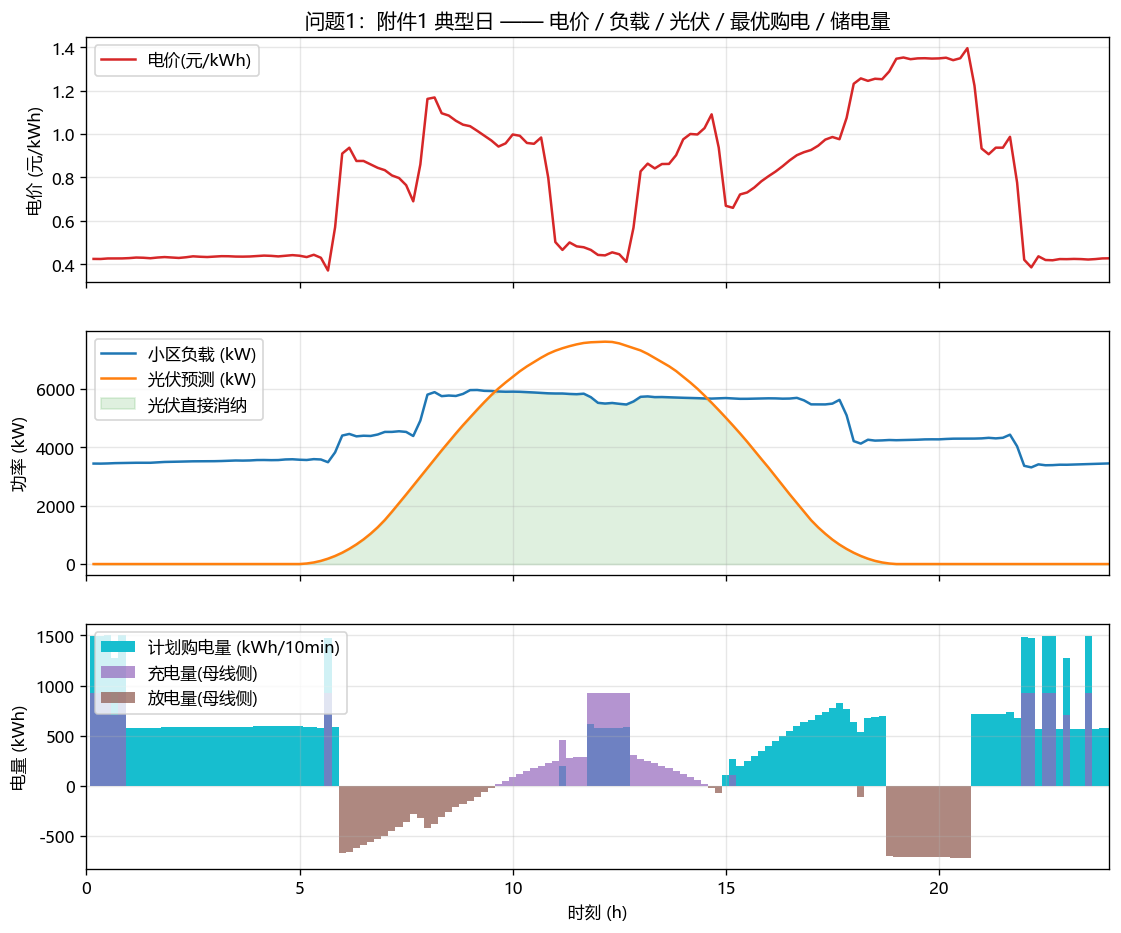
\includegraphics[width=0.42\textwidth]{../求解/图片/图1_问题1_最优购电与充放电策略.png}
  \caption{自检插图（测试中文与空格路径）}\label{fig:f}
\end{figure}

\section{代码与列表}
\begin{lstlisting}[language=Python,basicstyle=\ttfamily\small]
import numpy as np
print("hello CUMCM")
\end{lstlisting}
\cref{eq:e} 为储能动态方程。
\end{document}
